\documentclass[journal]{IEEEtran}
% \documentclass[conference]{IEEEtran}
% \IEEEoverridecommandlockouts
% The preceding line is only needed to identify funding in the first footnote. If that is unneeded, please comment it out.
\usepackage{amsmath,amssymb,amsfonts}
\usepackage{pifont}% http://ctan.org/pkg/pifont
\usepackage{algorithmic}
\usepackage{graphicx}
\usepackage{textcomp}
\usepackage{xcolor}
\usepackage{multirow}
\usepackage{array}
\usepackage[font=small, labelfont=bf]{subfig}
\usepackage[style=ieee, autocite=inline]{biblatex}
\addbibresource{ZoteroLibrary.bib}

\DeclareMathOperator*{\argmin}{\arg\!\min}
\newcommand{\cmark}{\ding{51}}%
\newcommand{\xmark}{\ding{55}}%
\newcolumntype{C}[1]{>{\rule{0pt}{3ex}\centering\arraybackslash}m{#1}} % define new column type


\begin{document}

\title{Discrete-time Control Contraction Metrics (DCCM) for Quasistatic Planar Pushing using Smoothed Dynamics\\
{\footnotesize MIT 2.152[J] Nonlinear Control Project Report}
}

\author{\IEEEauthorblockN{Shao Yuan Chew Chia}
\IEEEauthorblockA{
\textit{Harvard University}\\
Cambridge, MA \\
shaoyuan\_chewchia@college.harvard.edu
}}

\maketitle

\begin{abstract}

\end{abstract}

\section{Introduction}
% Control through contact is important
Planning and control through contact is an important capability in robotics. In order for robots to manipulate objects in their environment, they need to be able to reason about how to make and break contact. However, this has proved challenging for model-based methods due to two factors, namely, the non-smooth or hybrid nature of contact dynamics, as well as the underactuatedness of the system.

% Why control through contact is difficult - non smooth dynamics
Contact dynamics involve different modes of contact (e.g. sticking, sliding, no-contact), each with smooth but different dynamics and constraints. When switching between modes, the dynamics are discontinuous and change abruptly. This poses problems for gradient-based methods such as optimal control, as their locally linear models constructed using gradients quickly become inaccurate \autocite{pangGlobalPlanningContactRich2023}.
% Why control through contact is difficult - underactuated
Systems that involve contact are underactuated as the state of the unactuated objects cannot be controlled directly. Instead, control inputs to the robot are mediated through friction cones at contact points between the robot and the object, thus severely limiting the control authority of the inputs.

% Current methods for control through contact
Current methods for model based planning and control through contact typically fall into one of three categories: methods that apply smoothing to the dynamics \autocite{stewartOptimalControlSystems2010,pangGlobalPlanningContactRich2023}, methods that explicitly enumerate the contact modes \autocite{hoganFeedbackControlPusherSlider2016}, and methods that implicitly reason about the contact modes \autocite{sleimanContactImplicitTrajectoryOptimization2019,nakatsuruImplicitContactRichManipulation2023,posaDirectMethodTrajectory2014}. In this paper we apply these same smoothing techniques to explore the controllers that this enables.

% Why we would want to use Control Contraction Metrics
convex synthesis of contraction metric and controller, which we have powerful tools for like SOS programming.

The same controller exponentially stabilizes to arbitrary, time-varying feasible trajectories, while Lyapnov-based approaches typically need to be designed for a specific equilibrium.

provide guarantees on stability and convergence rates

% CCMs for underactuated systems
This work builds on \autocite{manchesterUnifyingRobotTrajectory2018} which demonstrates the effectiveness of CCMs on cannonical underactuated systems such as Cart-Pole.

% CCMs for discrete time
as well as \autocite{weiControlContractionMetric2021} that extends work in \autocite{manchesterControlContractionMetrics2017} to discrete time.

\section{Preliminaries and Problem Formulation}
\subsection{Quasistatic Assumptions}
We will assume that our system is quasistatic, meaning at each time step velocities and accelerations of the system are 0. This corresponds to having a high amount of damping and is a reasonable assumption in the 2D planar pushing setup where we restrict pushing velocities to be low and there is a large amount of friction between the object and table surface. As a result, the state of our system only consists of positions.

\subsection{Analytically Smoothed Contact Dynamics}
In this work we use the analytically smoothed contact dynamics and corresponding simulator developed by \autocite{pangGlobalPlanningContactRich2023}. Contact dynamics are formulated as an unconstrained convex program where the contact and friction contraints are moved into the objective function using a log barrier function. The effect of this is that there is a log barrier penalty for violating the contact constraints. Constraints can exert force even if they are not active and this translates to producing a force at a distance.

We plot the force at a distance effect of the smoothed contact dynamics in Figure \ref{fig:smoothed_contact_dynamics}. We see that for a high weight, which corresponds to a small force at a distance, the next $b_x$ is close to 0, but as the log barrier weight decreases, the box is pushed further to the right.

% Figure showing force at a distance
\begin{figure}[t]
	\centering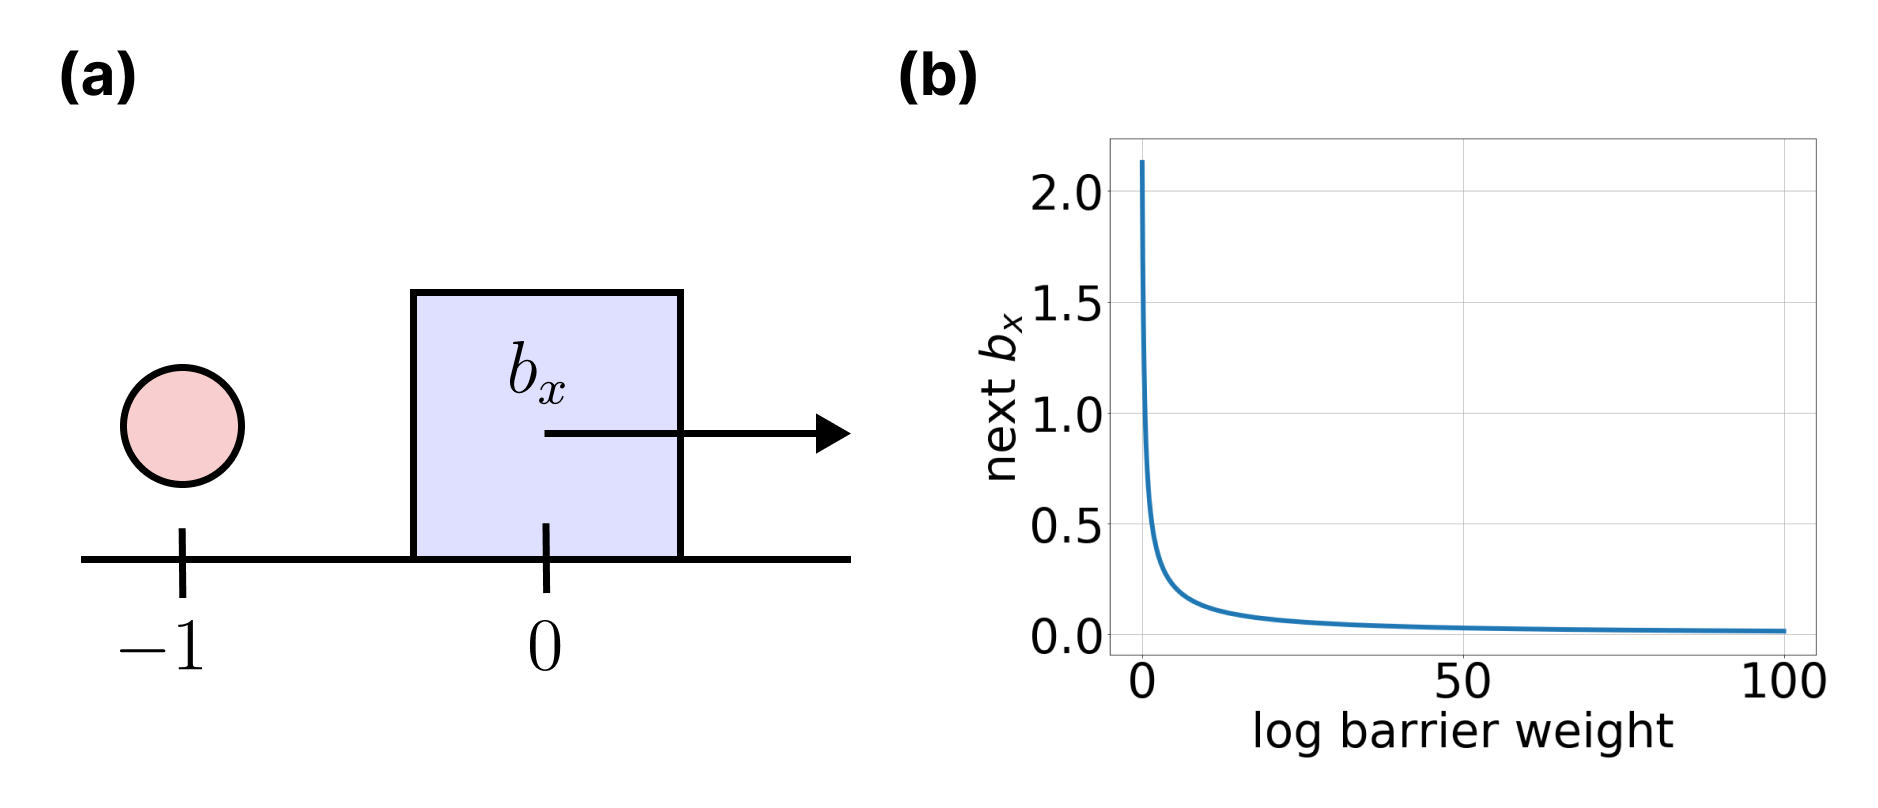
\includegraphics[width = 0.45 \textwidth]
	{figures/smoothed_contact_dynamics.png}
    \caption{Force at a distance effect of smoothed contact dynamics. (\textbf{a}) A system consisting of an actuated point finger at $x=-1$ and unactuated box at $x=0$, (\textbf{b}) The next $b_x$ after rolling out one step of the analytically smoothed dynamics with different log barrier weights.}
	\label{fig:smoothed_contact_dynamics}
	\vskip -0.25 true in
\end{figure}

\subsection{Planar Pushing System}
The state of 
\begin{equation}
    x = \begin{bmatrix}b_x & b_y & b_{\theta}& s_x& s_y\end{bmatrix}^\top
\end{equation}

control input $u$ are absolute position commands for the sphere
\begin{equation}
    u = \begin{bmatrix}u_x\\ u_y \end{bmatrix}
\end{equation}

The system evolves in nonlinearly in discrete time and is control affine. The dynamics are defined as

\begin{equation}
    x_{k+1} = f(x_k) + g(x_k)u_k
\end{equation}

where $f$ and $g$ are smooth functions due to the smoothing of the contact dynamics described in the previous section.

The differential dynamics are defined as
\begin{equation}
    \delta_{x_k} = A(x_k)\delta_{x_k} + B(x_k)\delta_{u_k}
\end{equation}
where $A(x_k) = \frac{\partial (f(x_k) + g(x_k)u_k)}{\partial x_k} \in \mathbb{R}^{5 \times 5}$ and $B(x_k) = \frac{\partial (f(x_k) + g(x_k)u_k)}{\partial u_k} \in \mathbb{R}^{5 \times 2}$ are the Jacobians of the dynamics.

We can define the state feedback control law
\begin{equation}
	\label{eq:delta_control_law}
    \delta_{u_k} = K(x_k)\delta_{x_k}
\end{equation}
where $K$ is the state dependent feedback gain matrix.

Generalized infinitesimal squared distance in the positive definite metric $M$ is denoted $V_k$
\begin{equation}
    V_k = \delta^\top_{x_k} M_{k} \delta_{x_k}
\end{equation}

And by substituting the differential dynamics and control law, we can see that the generalized infinitesimal squared distance at the next time step is

\begin{equation}
	\begin{aligned}
	V_{k+1} & = \delta^\top_{x_{k+1}} M_{k+1} \delta_{x_{k+1}} \\
	& = \delta^\top_{x_k} (A_k + B_k K_k)^\top M_{k+1} (A_k + B_k K_k)\delta_{x_k}
	\end{aligned}
\end{equation}

The contraction condition can then be expressed as
\begin{equation}
	V_{k+1} - V_k \leq 
	- \beta V_k <
	0
\end{equation}

which simplifies to
\begin{equation}
	\label{eq:contraction_condition}
	(A_k + B_k K_k)^\top M_{k+1} (A_k + B_k K_k) - (1 - \beta) M_k < 0
\end{equation}

\autocite{weiControlContractionMetric2021} showed that equation \ref{eq:contraction_condition} can be transformed via Schur's complement (among other transformations) into
% Create a 2x2 matrix
\begin{equation}
	\label{eq:contraction_condition_schur}
	\begin{bmatrix}
		W_{k+1} & A_k + B_k L_k \\
		(A_k + B_k L_k)^\top & (1 - \beta) W_k
	\end{bmatrix} > 0
\end{equation}
where $W := M^{-1}$ and $L := KW$

\section{Methods}
\subsection{Contraction Metric and Controller Synthesis}
\subsubsection{Sum of Squares (SOS) Programming}
In order to synthesize the contraction metric and controller, we use the SOS programming framework described in \autocite{weiControlContractionMetric2021} with some slight modifications.

\begin{equation}
	\label{eq:dccm_opt}
	\begin{aligned}
	\min_{l_c, w_c, r} & r \\
	s.t. & \forall k, w^\top \Omega w - r w^\top w \in \Sigma(x_k, u_k, w) \\
	& r \geq 0.1
	\end{aligned}
\end{equation}

where $\Sigma(x_k, u_k, w)$ is the set of SOS polynomials that satisfy the contraction condition in equation \ref{eq:contraction_condition_schur}. $l_c$ are the polynomial coefficients of $L$ and $w_c$ are the polynomial coefficients of $W$.
\begin{equation} 
	\begin{aligned}
	\Omega &=
	\begin{bmatrix}
		W_{k+1} & A_k + B_k L_k \\
		(A_k + B_k L_k)^\top & (1 - \beta) W_k
	\end{bmatrix} \\
	% W_k is a 5x5 symmetric matrix
	W_k &= 
	\begin{bmatrix}
		W_{11_k} & W_{12_k} & W_{13_k} & W_{14_k} & W_{15_k} \\
		W_{12_k} & W_{22_k} & W_{23_k} & W_{24_k} & W_{25_k} \\
		W_{13_k} & W_{23_k} & W_{33_k} & W_{34_k} & W_{35_k} \\
		W_{14_k} & W_{24_k} & W_{34_k} & W_{44_k} & W_{45_k} \\
		W_{15_k} & W_{25_k} & W_{35_k} & W_{45_k} & W_{55_k} \\
	\end{bmatrix} \\
	% L_k is a 2x5 matrix
	L_k &=
	\begin{bmatrix}
		L_{11_k} & L_{12_k} & L_{13_k} & L_{14_k} & L_{15_k} \\
		L_{21_k} & L_{22_k} & L_{23_k} & L_{24_k} & L_{25_k} \\
	\end{bmatrix} \\
	\end{aligned}
\end{equation}

each $W.._{k} = w.._c v(x_k)$ is a polynomial constructed from the row vector of coefficients of $w.._c$ and the monomial basis vector $v(x_k)$. For example, if the degree of the polynomial is chosen to be $4$,
\begin{equation}
	v(x_k) = [x^4_{k_4}, x_{k_3}x^3_{k_4}, x^2_{k_3}x^2_{k_4}, \cdots ,x_{k_1}, x_{k_0}, 1]
\end{equation}
where $v(x_k)$ has $126$ elements. $L.._k = l.._c v(x_k)$ is similarly defined.

In general, the dimensions of the matrices are as follows: $\Omega: 2 \cdot dim(x) \times 2 \cdot dim(x), W: dim(x) \times dim(x), L: dim(u) \times dim(x)$

We note the difference in the way we use the slack variable $r$ compared to \autocite{weiControlContractionMetric2021}. In \autocite{weiControlContractionMetric2021}, the constraints on the optimization program are $w^\top \Omega w - r I \in \Sigma(x_k, u_k, w), r \geq 0$. In practice we found that in some cases, especially when generating a higher degree metric, that the solver would return a trivial solution where $r$, $w_c$ and $l_c$ are extremely small numbers (on the order of $1e-17$). By setting a higher bound on $r$, we force the solver to find a solution where the contraction condition is satisfied with a greater buffer and the returned coefficients of $w_c$ and $l_c$ are larger.

Another difference is that we do not have closed form equations for the $A$ and $B$ matrices which would allow us to enforce the contraction conditions over all states. Instead, we sample a set of state, control action pairs and enforce the contraction condition over these samples. We use the contact dynamics solver described in \autocite{pangGlobalPlanningContactRich2023} to calculate the next state $x_{k+1}$, and the Jacobians $A_k$ and $B_k$, for each sample of the current state $x_k$ and control action $u_k$, and substitute these values into the constraints in optimization program (\ref{eq:dccm_opt}). Since $M$ is smooth, we can expect the contraction condition to be satisfied over at least a small local region around each sample. However, if the samples are too sparse, the contraction condition may not be satisfied over all the states around the desired trajectory.

We solve this SOS program using Drake's Mathematical Program \autocite{DrakeModelBasedDesign}, which uses Mosek under the hood to solve this Semidefinite Program (SDP).

\subsubsection{Sampling Strategy}
To get a contraction metric valid over the entire state space we would have to densely sample the entire state space. However, the available RAM on the machine sets an upper bound of the size of the optmization program, which for a monomial basis of degree $4$, was around $2000$ samples. Thus, to get a contraction metric and controller that had good performance at least in the vicinity of the desired trajectory, we only sampled states and control actions from a small region around the desired trajectory. This is a clear limitation of the current approach and future work would involve finding a way to enforce the contraction condition over a larger portion of state space.

\subsection{Online Geodesic and Controller Computation}
With the contraction metric synthesized, we now need to compute the control action that enforces the contraction condition.

For a smooth curve $c(s), s\in [0, 1]$ that connects two points in state space $x_0$ and $x_1$, \autocite{manchesterControlContractionMetrics2017} defines the Riemannian length and energy of the curve as

\begin{equation}
	\begin{aligned}
		L(c) &= \int_0^1 \sqrt{\frac{\partial{c(s)}}{\partial{s}} ^\top M(c(s)) \frac{\partial{c(s)}}{\partial{s}}} ds \\
		E(c) &= \int_0^1 L(c)^2 ds
	\end{aligned}
\end{equation}

The geodesic $\gamma(x_0, x_1)$ is the curve that minimizes the Riemanian length and energy between $x_0$ and $x_1$

\begin{equation}
	\label{eq:geodesic}
	\begin{aligned}
		\gamma(x_0, x_1) &= \argmin_{c} L(c) \\
		&= \arg \min_{c} E(c)
	\end{aligned}
\end{equation}

By the contraction condition we enforced, we see that the Riemanian energy of geodesic decreases exponentially as the system evolves and thus can be thought of as an incremental Lyapunov function \autocite{manchesterControlContractionMetrics2017}. In order to numerically approximate the geodesic $\gamma(x^*_k, x_k)$, we discretize the curve into $N$ segments and solve the following optimization program

\begin{equation}
	\label{eq:geodesic_opt}
	\begin{aligned}
		\bar{\gamma}(x^*_k, x_k) = \argmin_{ \substack{ x[\cdot], \Delta x_{s}[\cdot],\\ \Delta s[\cdot], m[\cdot], y[\cdot]}}
		& \sum_{i=0}^{N-1} y[i] + \Delta s[i]^2 \\
		s.t. & \forall i, y \geq \Delta s[i] \Delta x_s[i]^\top M(m[i]) \Delta x_s[i]\\
		& x[0] = x^*_k, \quad x[N] = x_k \\
		& \forall i, x[i+1] = x[i] + \Delta x_{s}[i]\Delta s[i] \\
		& \forall i, \Delta s[i] > 0, \quad \sum_{i=0}^{N-1} \Delta s[i] = 1\\
		& \forall i, M(m[i]) W(x[i]) = I  \\
	\end{aligned}
\end{equation}
where $x[i]$ is the state at the start of the $i$th segment of the geodesic, $\Delta s[i]$ is a small positive scalar, $\Delta x_s[i]$ is the discretized displacement vector, $y[i]$ is a slack variable that represents the Riemanian energy and $N$ is the number of segments the $\gamma$ is discretized into. $m[i]$ is a slack variable introduced such that the $5\times5$ symbolic matrix $W(x[i])$ does not need to be explicitly inverted which was found to be a severe computational bottleneck. The constraint $M(m[i]) W(x[i]) = I$ is a surrogate for enforcing $M(m[i])=W(x[i])^{-1}$. Adding $\Delta s[i]^2$ to the objective serves to spread out the discretized points evenly along the geodesic.

As this is a non-convex program, we use Drake, this time using SNOPT under the hood \autocite{DrakeModelBasedDesign}.

With the geodesic $\bar{\gamma}(x^*_k, x_k)$ computed, we can compute the control action $u_k$ that enforces the contraction condition

\begin{equation}
	\label{eq:control_law}
	\begin{aligned}
		u_k &= u^*_k + \sum_{i=0}^{N-1} \Delta s[i] K(x[i]) \Delta x_s[i]  \\
		&= u^*_k + \sum_{i=0}^{N-1} \Delta s[i] L(x[i]) W(x[i])^{-1} \Delta x_s[i]
	\end{aligned}
\end{equation}

An important point to note is that the integration is done from $x^*_k$ to $x_k$ and not the other way around. While it might seem intuitive that we want to calculate the $\delta_u$ that brings the system from $x_k$ to $x^*_k$, this is actually not the right way to think about it. First, the $\delta_u$ in equation \ref{eq:delta_control_law} does not lead to a change in state $\delta_x$ on the right side of the same equation. Instead, \ref{eq:delta_control_law} tells us for a change in state $\delta_x$ from a nominal trajectory, what is the corresponding $\delta_u$ that enforces the contraction condition. In this case, the nominal trajectory is $x^*$ and $u^*$, thus to calculate the $\delta_u$ that enforces the contraction condition, we need to integrate from $x^*_k$ to $x_k$.

\section{Experimental Setup}
\subsection{Creating Feasible Desired Trajectories}
To create the desired trajectory, we first parameterised an arbitrary circular trajectory with the robot "behind" the object at each time step and the object slowly rotating as it travelled around the circle. We then rolled out the dynamics from the initial condition, using the position of the robot at the next time step as the open loop position command for the robot and recorded the actual positions of the object under this open loop control. We created two feasible circular trajectories of slightly different radius in this way and spliced them together in the middle in order to introduce a step change in the desired trajectory. Finally, we introduce an additional initial disturbance by adding an offset to the initial state from the first state of the desired trajectory. We do this process twice to create desired trajectories for both the log barrier weight 10 and 100 levels of smoothing.

\section{Results and Discussion}
Our original goal was to synthesize a DCCM with a small amount of smoothing that would transfer well to stabilizing the real system to arbitrary feasible desired trajectories under non-smooth, exact contact dynamics. Unfortunately, we were not able to achieve this goal. We find that when using a small amount of smoothing, a higher degree monomial basis was required to enforce the contraction condition across all samples. Furthermore, since the dynamics were less smooth, a greater density of samples was required in order for the contraction condition to hold around the desired trajectory. This can be seen from the result in table (\ref{table:results_overview}) where even though we were able to synthesize DCCMs for 500 samples for both log barrier weights, the DCCM for log barrier weight 10 worked while the DCCM for log barrier weight 100 did not.

Both of these factors (requiring a higher degree, and more samples) led to the optimization (\ref{eq:dccm_opt}) being intractable due to the computer used running out of RAM. Ultimately we were only able to find a stabilizing controller for a log barrier weight of 10, which corresponds to the robot exerting $0.1$ Newtons of force on an object that is $1$ meter away.

\begin{table}[thpb]
	\centering
	\begin{tabular}{| C{0.8cm} | c | c || c | c | c | c | c |} 
		\hline
		Log Barrier Weight  & Deg. & \# Samples 
		& 100 &500 & 1000 & 2000 & 3000\\ \hline\hline
		\multirow{4}{*}{10} & \multirow{2}{*}{4} 
		& Synthesizes 
		& \cmark & \cmark & \cmark & \cmark & ! \\ \cline{3-8}
		& & Stabilzes 
		& \xmark & \cmark & \cmark & \cmark & - \\ \cline{2-8}
		& \multirow{2}{*}{6}
		& Synthesizes 
		\\ \cline{3-8}
		& &  Stabilizes \\ \hline
		\multirow{4}{*}{100} & \multirow{2}{*}{4} 
		& Synthesizes
		& \cmark & \cmark & \xmark & - & - \\ \cline{3-8}
		& & Stabilzes
		& \xmark & \xmark & - & - & -\\ \cline{2-8}
		& \multirow{2}{*}{6} 
		& Synthesizes
		& \cmark & \cmark & ! & - & -\\ \cline{3-8}
		& &  Stabilizes
		& \xmark & \xmark & - & - & -\\ \hline
	\end{tabular}
	\caption{Feasibility (whether a DCCM can be synthesized) and performance (whether the found DCCM stabilizes to the desired trajectory) across different log barrier weights (10 is high smoothing, 100 is low smoothing), degree of monomial basis used, and number of sampled points at which the contraction condition is enforced.  Symbols: \cmark (succeeds), \xmark (fails), ! (program crashes), - (did not/could not run test).}
	\label{table:results_overview}
\end{table}

\subsection{Effect of different parameters}




\subsection{Degree of metric on}
Higher degree means its more able to find a contraction metric for a system with more "warped" dynamics, i.e. if there is less smoothing. 

But higher degree also means less samples can be used, and increased computation time.
\subsection{Effect of number of samples on controller performance}

\section{Conclusion and Future Work}
More work needs to be done to realize the full benefits of applying the Control Contraction Metric Framework to the problem of control through contact. 


Same controller across different trajectories - this was not realized in our implementation because of the sampling technique used.

Convex synthesis - high degree SOS polynomial required

Certificates of stability and convergence rates - need arguments about samping density, and also bounding the difference between smoothed and exact dynamics.

faster online computation - explore other methods for solving the geodesic that don't involve inverting the symbolic matrix.

\printbibliography

\end{document}
